%\documentclass[11pt,oneside,a4paper,openright]{report}
%\usepackage[utf8]{inputenc}
%\renewcommand{\contentsname}{Indholdsfortegnelse}
%\usepackage{pdfpages}
%\usepackage{titlesec}
%\titleformat{\chapter}{\normalfont\huge}{\thechapter.}{20pt}{\huge\it}

%%%% Dokumentklassen %%%%

\documentclass[a4paper,11pt,dvipsnames,oneside,openany]{memoir} 	% Openright åbner kapitler på højresider (openany begge)
% fleqn = flush left equation - sikre at alle ligninger tvinges til venstre. I 3. semesterprojektet, skulle ligningerne stå i midten derfor er denne pakke slettet fra dokumentklassen.

\usepackage{subfiles}
\usepackage{nameref}
\usepackage{tabularx}
\usepackage{multirow}
\usepackage[table]{xcolor}


%%%% PACKAGES %%%%

%% Oversættelse og tegnsætning %%
\usepackage[utf8]{inputenc}					% Input-indkodning af tegnsæt (UTF8)
\usepackage[danish]{babel}					% Dokumentets sprog
\usepackage[T1]{fontenc}				    % Output-indkodning af tegnsæt (T1)
\usepackage{ragged2e,anyfontsize}			% Justering af elementer
%\usepackage{fixltx2e}						% Retter forskellige fejl i LaTeX-kernen
\usepackage{titletoc}
\newcommand{\nocontentsline}[3]{}
\newcommand{\tocless}[2]{\bgroup\let\addcontentsline=\nocontentsline#1{#2}\egroup}									% Giver mulighed for at fjerne section nummer i indholdsfortegnelse ved \tocless


\usepackage{lastpage}						% Total antal sider opdateres automatisk ved \pageref{LastPage}
\usepackage{tikz}							% Til at lave flow diagrammer
\usetikzlibrary{calc,trees,positioning,arrows,chains,shapes.geometric,decorations.pathreplacing,decorations.pathmorphing,shapes,matrix,shapes.symbols}				% Til at lave diagrammer
																			
%% Figurer og tabeller (floats) %%
\usepackage{graphicx} 						% Håndtering af eksterne billeder (JPG, PNG, EPS, PDF)
\usepackage{multicol}         	           	% Muliggør output i spalter
\usepackage{rotating}						% Rotation af tekst med \begin{sideways}...\end{sideways}
\usepackage{xcolor}							% Definer farver med \definecolor. Se mere: http://en.wikibooks.org/wiki/LaTeX/Colors
\usepackage{flafter}						% Sørger for at floats ikke optræder i teksten før deres reference
\let\newfloat\relax 						% Justering mellem float-pakken og memoir
\usepackage{float}							% Muliggør eksakt placering af floats, f.eks. \begin{figure}[H]
\usepackage{color, colortbl}				% Tilføjer farve til tabeller

\definecolor{Gray}{gray}{0.9}				% Definerer en farve "yeezy-gray"

%% Matematik mm. %%
\usepackage{amsmath,amssymb,stmaryrd} 		% Avancerede matematik-udvidelser
\usepackage{mathtools}						% Andre matematik- og tegnudvidelser
\usepackage{textcomp}                 		% Symbol-udvidelser (fx promille-tegn med \textperthousand)
\usepackage{rsphrase}						% Kemi-pakke til RS-saetninger, fx \rsphrase{R1}
\usepackage[version=3]{mhchem} 				% Kemi-pakke til flot og let notation af formler, f.eks. \ce{Fe2O3}
\usepackage{siunitx}						% Flot og konsistent præsentation af tal og enheder med \si{enhed} og \SI{tal}{enhed}
\sisetup{output-decimal-marker = {,}}		% Opsætning af \SI (DE for komma som decimalseparator) 

%% Referencer og kilder %%
\usepackage[danish]{varioref}				% Muliggør bl.a. krydshenvisninger med sidetal (\vref)
\usepackage{natbib}							% Udvidelse med naturvidenskabelige citationsmodeller
\usepackage{xr}							    % Referencer til eksternt dokument med \externaldocument{<NAVN>}

%% Misc. %%
\usepackage{listings}						% Placer kildekode i dokumentet med \begin{lstlisting}...\end{lstlisting}
\usepackage{lipsum}							% Dummy text \lipsum[..]
\usepackage[shortlabels]{enumitem}			% Muliggør enkelt konfiguration af lister
\usepackage{pdfpages}						% Gør det muligt at inkludere pdf-dokumenter med kommandoen \includepdf[pages={x-y}]{fil.pdf}	
\pdfoptionpdfminorversion=6					% Muliggør inkludering af pdf-dokumenter, af version 1.6 og højere
\pretolerance=2500 							% Justering af afstand mellem ord (højt tal, mindre orddeling og mere luft mellem ord)


%%%% CUSTOM SETTINGS %%%%

%% Marginer %%
\setlrmarginsandblock{3.0cm}{3.0cm}{*}		% \setlrmarginsandblock{Indbinding}{Kant}{Ratio}
\setulmarginsandblock{3.0cm}{3.0cm}{*}		% \setulmarginsandblock{Top}{Bund}{Ratio}
\checkandfixthelayout 						% Oversætter værdier til brug for andre pakker

%% Afsnitsformatering %%
\setlength{\parindent}{0mm}           		% Størrelse af indryk
\setlength{\parskip}{3mm}          			% Afstand mellem afsnit ved brug af double Enter
\linespread{1,1}							% Linjeafstand

%% Indholdsfortegnelse %%
\setsecnumdepth{subsection}		 			% Dybden af nummererede overskrifter (part/chapter/section/subsection)
\maxsecnumdepth{subsection}					% Dokumentklassens grænse for nummereringsdybde
\settocdepth{subsubsection} 					% Dybden af indholdsfortegnelsen
\setcounter{secnumdepth}{5} 				    % Ekstra subsubsection nummerering
		
%% Opsætning af listings %%
\definecolor{commentGreen}{RGB}{34,139,24}
\definecolor{stringPurple}{RGB}{208,76,239}

\lstset{language=Matlab,				    % Sprog
	basicstyle=\ttfamily\scriptsize,	    % Opsætning af teksten
	keywords={for,if,while,else,elseif,		% Nøgleord at fremhæve
			  end,break,return,case,
			  switch,function},
	keywordstyle=\color{blue},				% Opsætning af nøgleord
	commentstyle=\color{commentGreen},		% Opsætning af kommentarer
	stringstyle=\color{stringPurple},		% Opsætning af strenge
	showstringspaces=false,					% Mellemrum i strenge enten vist eller blanke
	numbers=left, numberstyle=\tiny,		    % Linjenumre
	extendedchars=true, 					    % Tillader specielle karakterer
	columns=flexible,						% Kolonnejustering
	breaklines, breakatwhitespace=true,		% Bryd lange linjer
}

%% Navngivning %%
\addto\captionsdanish{
	\renewcommand\appendixname{Appendiks}
	\renewcommand\contentsname{Indholdsfortegnelse}	
	\renewcommand\appendixpagename{Appendiks}
	\renewcommand\appendixtocname{Appendiks}
	\renewcommand\cftchaptername{\chaptername~}		% Skriver "Kapitel" foran kapitlerne i indholdsfortegnelsen
	\renewcommand\cftappendixname{\appendixname~}	% Skriver "Appendiks" foran appendiks i indholdsfortegnelsen
}

%% Kapiteludssende %%
\definecolor{numbercolor}{gray}{0.7}		            % Definerer en farve til brug til kapiteludseende
\newif\ifchapternonum

\makechapterstyle{jenor}{					        % Definerer kapiteludseende frem til ...
  \renewcommand\beforechapskip{0pt}
  \renewcommand\printchaptername{}
  \renewcommand\printchapternum{}
  \renewcommand\printchapternonum{\chapternonumtrue}
  \renewcommand\chaptitlefont{\fontfamily{pbk}\fontseries{db}\fontshape{n}\fontsize{25}{35}\selectfont\raggedleft}
  \renewcommand\chapnumfont{\fontfamily{pbk}\fontseries{m}\fontshape{n}\fontsize{1in}{0in}\selectfont\color{numbercolor}}
  \renewcommand\printchaptertitle[1]{%
    \noindent
    \ifchapternonum
    \begin{tabularx}{\textwidth}{X}
    {\let\\\newline\chaptitlefont ##1\par} 
    \end{tabularx}
    \par\vskip-2.5mm\hrule
    \else
    \begin{tabularx}{\textwidth}{Xl}
    {\parbox[b]{\linewidth}{\chaptitlefont ##1}} & \raisebox{-15pt}{\chapnumfont \thechapter}
    \end{tabularx}
    \par\vskip2mm\hrule
    \fi
  }
}											        % ... her

\chapterstyle{jenor}						        % Valg af kapiteludseende - Google 'memoir chapter styles' for alternativer

%% Sidehoved %%

\makepagestyle{AAU}							        % Definerer sidehoved og sidefod udseende frem til ...
\makepsmarks{AAU}{%
	\createmark{chapter}{left}{shownumber}{}{. \ }
	\createmark{section}{right}{shownumber}{}{. \ }
	\createplainmark{toc}{both}{\contentsname}
	\createplainmark{lof}{both}{\listfigurename}
	\createplainmark{lot}{both}{\listtablename}
	\createplainmark{bib}{both}{\bibname}
	\createplainmark{index}{both}{\indexname}
	\createplainmark{glossary}{both}{\glossaryname}
}
\nouppercaseheads									% Ingen Caps ønskes

\makeevenhead{AAU}{\small E17BAC-Synk2}{}{\leftmark}	% Definerer lige siders sidehoved (\makeevenhead{Navn}{Venstre}{Center}{Hoejre})
\makeoddhead{AAU}{\rightmark}{}{}		            % Definerer ulige siders sidehoved (\makeoddhead{Navn}{Venstre}{Center}{Højre})
\makeevenfoot{AAU}{\small \thepage \ }{}{ }						% Definerer lige siders sidefod (\makeevenfoot{Navn}{Venstre}{Center}{Højre})
\makeoddfoot{AAU}{}{}{\small \thepage \ }						% Definerer ulige siders sidefod (\makeoddfoot{Navn}{Venstre}{Center}{Højre})

\copypagestyle{AAUchap}{AAU}							% Sidehoved for kapitelsider defineres som standardsider, men med blank sidehoved
\makeoddhead{AAUchap}{}{}{}
\makeevenhead{AAUchap}{}{}{}
\makeheadrule{AAUchap}{\textwidth}{0pt}
\aliaspagestyle{chapter}{AAUchap}					% Den ny style vælges til at gælde for chapters
													% ... her
															
\pagestyle{AAU}										% Valg af sidehoved og sidefod


%%%% CUSTOM COMMANDS %%%%

%% Billede hack %%
\newcommand{\figur}[4]{
		\begin{figure}[H] \centering
			\includegraphics[width=#1\textwidth]{billeder/#2}
			\caption{#3}\label{#4}
		\end{figure} 
}

%% Specielle tegn %%
\newcommand{\decC}{^{\circ}\text{C}}
\newcommand{\dec}{^{\circ}}
\newcommand{\m}{\cdot}


%%%% ORDDELING %%%%

\hyphenation{}


%%%% Tilføjelser af min preample %%%%

% Booktabs:
% The booktabs package is needed for better looking tables. 
\usepackage{booktabs}

% Caption:
% For better looking captions. See caption documentation on how to change the format of the captions.
\usepackage[hang, font={small, it}]{caption}

% Hyperref:
% This package makes all references within your document clickable. By default, these references will become boxed and colored. This is turned back to normal with the \hypersetup command below.
\usepackage{hyperref}
	\hypersetup{colorlinks=false,pdfborder=0 0 0}

% Cleveref:
% This package automatically detects the type of reference (equation, table, etc.) when the \cref{} command is used. It then adds a word in front of the reference, i.e. Fig. in front of a reference to a figure. With the \crefname{}{}{} command, these words may be changed.
\usepackage{cleveref}
	\crefname{equation}{formel}{formler}
	\crefname{figure}{figur}{figurer}	
	\crefname{table}{tabel}{tabeller}

% Mine tilføjelser:
\usepackage{units}                        %% Bruges til at gøre fx 1/2 samlet med: \nicefrac{1}{2}.
\usepackage{tabu, longtable}              %% Bruges til tabeller.
\setlength{\tabulinesep}{1.5ex}           %% Definerer linjeafstand i tabeller.
\usepackage{enumerate}                    %% Bruges til lister.
\usepackage{tabto}                        %% Giver mulighed for TAB med fx \tabto{3em}.
\usepackage[hyphenbreaks]{breakurl}       %% Bruges til websiders url'er.
\renewcommand{\UrlFont}{                  %% Definerer url-font.
\small\ttfamily}                          %
\bibliographystyle{unsrt}                 %% Definere bibliografien. Ses til sidst i dokumentet i kapitlet Litteratur.
\usepackage{amssymb} 
\usepackage{pifont}
%\newcommand{\xmark{\ding{55}}			 % Opretter et unchecked mark

\usepackage[bottom]{footmisc}

\usetikzlibrary{%
    decorations.pathreplacing,%
    decorations.pathmorphing,%
    arrows,
    arrows.meta,
    positioning,
    shapes,
    shadows,
    shapes.geometric
    }
    \usepackage{relsize}

%\definecolor{myblue1}{RGB}{0,157,209}
\definecolor{myblue1}{rgb}{0.12, 0.56, 1.0}
\definecolor{myblue3}{RGB}{216,229,245}
%\definecolor{myblue4}{RGB}{0,149,229}
\definecolor{myblue2}{rgb}{0.19, 0.55, 0.91}
\definecolor{myblue4}{rgb}{0.08, 0.38, 0.74}
\definecolor{myred1}{rgb}{0.82, 0.1, 0.26}
\definecolor{myyellow1}{rgb}{1.0, 0.96, 0.0}
\definecolor{myyellow2}{rgb}{1.0, 0.65, 0.0}


\usepackage{pdflscape}
\usepackage{rotating}

\begin{document}
\begin{titlingpage}
\begin{center}

~ \\[3cm]

%\includegraphics[width=0.6\textwidth]{figurer/ASE}~\\[1cm]
\textsc{\LARGE Bilag 6}\\[1.5cm]

%\textsc{\Large Sundhedsteknologi}\\
%\textsc{\Large 3. semesterprojekt}\\[0.5cm]

\noindent\makebox[\linewidth]{\rule{\textwidth}{0.4pt}}\\
[0.5cm]{\Huge Design}
\noindent\makebox[\linewidth]{\rule{\textwidth}{0.4pt}}
\end{center}
\vfill
\begin{center}
{\large 19. december 2017}
\end{center}
\end{titlingpage}

\newpage
\tableofcontents*
\newpage

\chapter{Indledning}
I dette bilag forklares design af hardware og software  for synkerefleksmonitoren. På baggrund af HW-arkitekturen redegøres der, hvordan HW-blokkene, som indgår i HW-arkitekturen er designet samt deres funktion. Desuden indeholder afsnittet en kort beskrivelse af designovervejelser i forhold til de enkelte hardwareenheder. Figur \ref{blokflow} viser de komponenter, som skal anvendes for at synkerefleksmonitoren kan blive realiseret. Nogle af disse komponenter skal designes af gruppens medlemmer mens  resten er kommercielle komponenter, der anvendes pga. deres specifikationer. Disse kommercielle komponenter omfatter en Analog Discovery, en PC og en EMG-måler. Dette afsnit forholder sig ikke til design disse kommercielle komponenter, men om de kan leve op til de krav som er nødvendig for at realisere det ønskede produkt. Desuden indeholder bilaget et sekvens diagram, der  giver en detaljeret beskrivelse af udvalgte funktioner/metoder, som styrer synkerefleksmonitorens hardware del.   

\begin{figure}[H]
\centering
{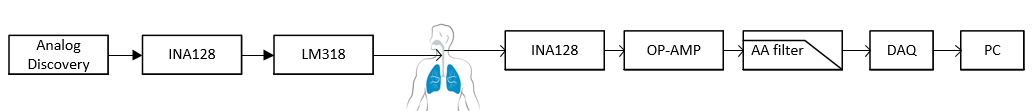
\includegraphics[width=\linewidth]
{Figure/Blokaede}}
\caption{Figuren viser de enkelte komponenter, som skal designes for at realisere synkerefleksmonitoren.}
\label{blokflow}
\end{figure}


\chapter{Hardware}

\subsection{Analog Discovery}
Analog Discovery (AD) bruges i dette projekt til to formål. Det første er at AD skal fungere som funktionsgenerator og det andet er at den den skal også fungere som dataopsamlingmodul. Figur \ref{ToINA128} viser et skitse af de to formål som AD bliver brugt til. Her ses det at AD generere et AC signal på 2V, som sendes til indgangen af instrumentationsforstærkeren INA128. Dette signal bliver brugt til at generere en konstant strøm ud af operationsforstærkeren LM318. Det ses også på figuren at AD modtager et signal fra et antialiaseringsfilter. Her fungerer AD en dataopsamlingsmodul, der konverter et analog signal til et digital signal. 


   
\begin{figure}[H]
\centering
{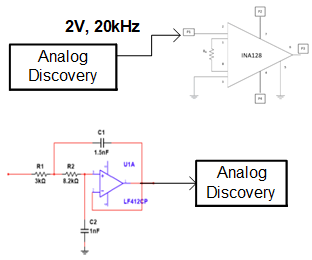
\includegraphics[width=\linewidth]
{Figure/ADogINA128}}
\caption{Figuren viser ADs funktion i det samlede system. AD fungerer som funktionsgenerator og som dataopsamlingsmodul}
\label{analogOgINA}
\end{figure}


For at rekonstruere et fysiologisk signal som eksisterer i et analog domæne til et digital domæne kræver det at man opfylder en række krav. Den første krav er at overholde Shannons samplingsteorem som siger at samplingsfrekvensen skal minimum være 2 gange den maksimale frekvenskomponent, Nyquist-frekvensen. I praksis ønsker man en måling, der ikke indeholder frekvenser, som er større end den halve samplingsfrekvens dvs. Nyquist-frekvensen. Frekvenser større end Nyquist-frekvensen giver anledning til aliasering, der gør det vanskeligt at rekonstruere det oprindelige signal korrekt. For at genskabe et signal bedst muligt anbefales det at man vælger en samplingsfrekvens, der er betydelig højere end den maksimale frekvenskomponent. Valg af dataopsamlingsenhed har også betydning for hvor præcise man kan genskabe et analog signal. Konvertering af analoge værdier til digitale værdier sker ved at dataopsamlingsenheden måler et analog signal værdi, som derefter konverteres til den nærmeste digital værdi. Under konvertering opstår der fejl, da konverteringen ikke er præcis, men approksimation. Denne fejl kaldes kvantiseringsfejl.  Konverteringens præcision bestemmes af ADC'ens spændingsområde og opløsning. Forholdet mellem ADC'ens inputområde og dens kvantificeringsniveauer/ADC’ens opløsning kan udtrykkes ved denne formel  \cite [s. 634-635]{Lyons}:

\begin{equation}
\label{eq2.1}
 LSB=  \dfrac{{Spændingsområde}}{2^{bits}} 
\end{equation}

Denne formel udtrykker A/D konverterens mindste detekterbare spændingsændring, Least Significant Bit. I dette projekt benyttes AD, der kan yde 14-bit analog til digital-konvertering og som får en spændingsforsyning på 8V. Med disse opløsninger kan LSB beregnes som følgende:

 \begin{equation}
\label{eq2.2}
 LSB=  \dfrac{{8V}}{2^{14}}=0,48mV 
\end{equation}
 
 Dette betyder at det mindste detekterbare spændingsændring som AD kan detektere er 0.48mV. Spændingsændringer over 0,48mV bliver omsæt til digitale værdier og værdier under den bliver ikke omsæt. AD er valgt ud fra følgende fordele:
 
 \begin{itemize}
\item 	Den kan fungere som funktionsgenerator samtidig med at den læser to signaler ind simultant
\item Den kan sample to signaler simultant med en $f_{s}=500000MHz $
\item Den kan fungere som dataopsamlingsenhed 
 
\end{itemize}
Med disse fordele er det besluttet at benytte AD. 
 
 \pagebreak

\subsection{Instrumentationsforstærker  1 og 2}
Når man måler fysiologiske signaler har man bruge for at forstærke dem, da deres amplituder er små. Disse amplituder skal forstærkes fra millivolt  til volt området. Ydermere er disse signaler overlejret med brum støj på 50 Hz, som kommer af de omkringliggende apparater, ved at måleudstyret og måleobjektet har elektromagnetisk kobling imellem hinanden. For at eliminere eller undertrykke denne støj mest muligt anvendes en differensforstærker. Udover at undertrykke denne støj, ønsker man også som omtalt at forstærke indgangssignalet fra funktionsgeneratoren. Derfor anvendes i dette projekt to instrumentationsforstærker af typen INA128P. Med INA128P er det muligt at forstærke et signal ved kun at regulere én modstand. Dette betyder at et ønsket forstærkning kan opnås ved at kun justere den eksterne modstand kaldet $(R_G)$. INA128P har følgende egenskaber som er ønskede, når man måler elektrofysiologiske signaler \textbf{Citer peters pdf}. 

\begin{itemize}
\item 	Høj indgangsimpedans på ca. $10^{10} \Omega $
\item	Stor common mode rejection (CMR) på minimum 120dB
\item 	Differentielt input-single ended out (nødvendigt for at mindske $CM_{noise}$)
\end{itemize}

I dette projekt implementeres to instrumentationsforstærker af typen INA128. Den ene bruges til at forstærke signalet fra funktionsgeneratoren og fjerne brum støj på 50Hz, og den anden anvendes til både at forstærke elektrofysiologiske signaler fra måleobjektet og undertrykkelse af commen mode støj.  

\begin{figure}[H]
\centering
{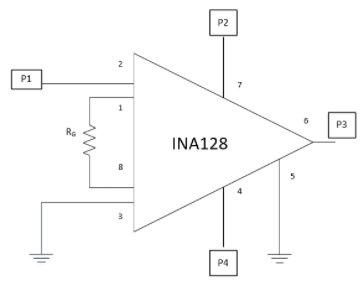
\includegraphics[width=\linewidth]
{Figure/Ina128Design}}
\caption{Figuren viser en instrumentationsforstærker. Den bruges til undertrykkelse af støj og forstærkning af fysiologiske signaler fra måleobjektet }
\label{ToINA128}
\end{figure}

Den ønskede forstærkning reguleres vha. $R_G$ og det kan udledes af denn formel:

\begin{equation}
\label{eq2.3}
Gain  =1 + \dfrac{{50k\Omega}}{R_G}
\end{equation}




Ved anvendelse af INA128 kan man forstærke et signal 100 gange og stadig have en tilstrækkelig båndbredde, der ligger over anti-aliaseringsfilterets knækfrekvens på $20kHz$. Dette kan aflæses på figur \ref{Fig:GainOgfrequnecy}. 

\begin{figure}[H]
\centering
{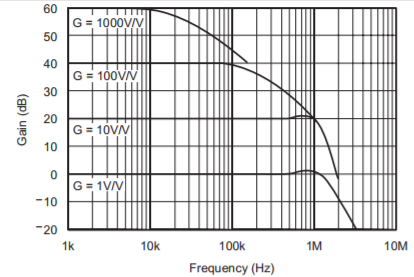
\includegraphics[width=\linewidth]
{Figure/GainOgfrequnecy}}
\caption{Figuren viser at Gain på 10V/V bliver ved at være konstant op til ca. 500kHz. Vælger man derimod gain på 100 V/V så er gain konstant kun op til ca. 100kHz \cite{TexasInstruments2005} }
\label{Fig:GainOgfrequnecy}
\end{figure} 

Det ses på figur \ref{Fig:GainOgfrequnecy} at båndbredden BW er større end anti-aliaseringsfilterets knækfrekvens på 20khz, når gain vælges til 100. Dette betyder at forstærkeren er bred nok til at kunne indeholde frekvenser, der er større og mindre end knækfrekvensen.  Med denne aflæsning af BW er det sikrede at INA128 kan benyttes til formålet. 


Ved at sætte Gain=100 kan man beregne $ R_{G}$

\begin{equation}
\label{eq2.4}
Gain = 100 $$ $$ \\
Gain  =100 + \dfrac{{50k\Omega}}{R_G} \Rightarrow {R_G}=505 \Omega
\end{equation}

For at teste om INA128 kan i praksis levere en gain på 100 laves der en spændingsdeler kredsløb, der modtager et signal på 1V, som derefter bliver formindsket til $10mV$. Dette spændingsdeler kredsløb er nødvendig pga:

\begin{itemize}
\item 	at man ikke direkte kan sende små signaler fra AD til INA128 pga. AD har store usikkerheder, når den genererer små signaler 
\item	at man ikke kan sende 1V igennem INA128 med gain på 100. Dette giver en udgangsspænding på 100V, som INA128 ikke kan klare. 

\end{itemize}

Med de to begrundelse designes følgende spændingsdeler kredsløb:


\begin{figure}[H]
\centering
{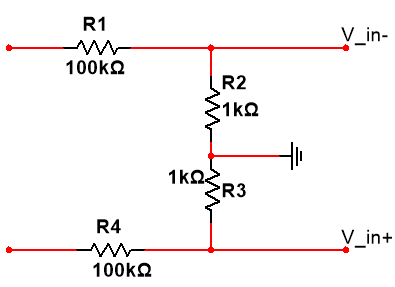
\includegraphics[width=\linewidth]
{Figure/spaedingdeler}}
\caption{Figuren viser kredsløbet til spændingsdeleren}
\label{Fig:GainOgfrequnecy}
\end{figure} 

\begin{equation}
\label{eq2.5}
V_{inINA128} = 10 \times 10^{-3}V $$ $$ \\
R_{1} = 100k\Omega, R_{2} =1000\Omega $$ $$ \\
V_{outIna128}  = 100 \times \dfrac{R_{2}}{R_{1}+ R_{2}}=1V
\end{equation}

Det forventes at INA128 forstærker 10mV til 1V, hvilken svar til en gain på 100.  


Da INA128 som nævnte også benyttes til at forstærke signalet fra funktionsgeneratoren på 2V, skal den eksterne modstand, $R_G$, også beregnes for denne. Hvis gain vælges til 2 skal man ifølge databladet  sætte $R_G=50k\Omega$  \citep [s.13]{TexasInstruments2005}. 
Udgangssignalet for denne instrumentationsforstærker   beregnes som den forudgående: 

\begin{equation}
\label{eq2.6}
V_{in} = 2 $$ $$
Gain = 2 $$ $$
V_{outINA128}=2V \times 2=4V
\end{equation}

Med en kendt Gain kan der nu beregnes $R_G$:


\begin{equation}
\label{eq2.7}
Gain = 2 $$ $$ \\
Gain  =2 + \dfrac{{50k\Omega}}{R_G} \Rightarrow {R_G}=50k \Omega
\end{equation}

\subsection{Strømgenerator}

Da bioimpedans måling kræver at man sender en konstant strøm til måleobjektets væv er det nødvendigt at designe og opbygge en strømgenerator, der kan levere en konstant strøm. Som beskrevet\textbf{ i analyse afsnittet er der testet og sammenlignet to operationsforstærker}, som kan anvendes til dette formål. Testen har vist at operationsforstærkeren LM118 er bedre til at levere en konstant strøm, når vævsmodstanden varieres. Derfor vælges LM118 til at levere det ønsket strøm frem for den anden operationsforstærker LF412N. Det forventet strømoutput som LM118 leverer til vævet, når $R_4 =10k\Omega $, kan beregnes som følgende:

\begin{figure}[H]
\centering
{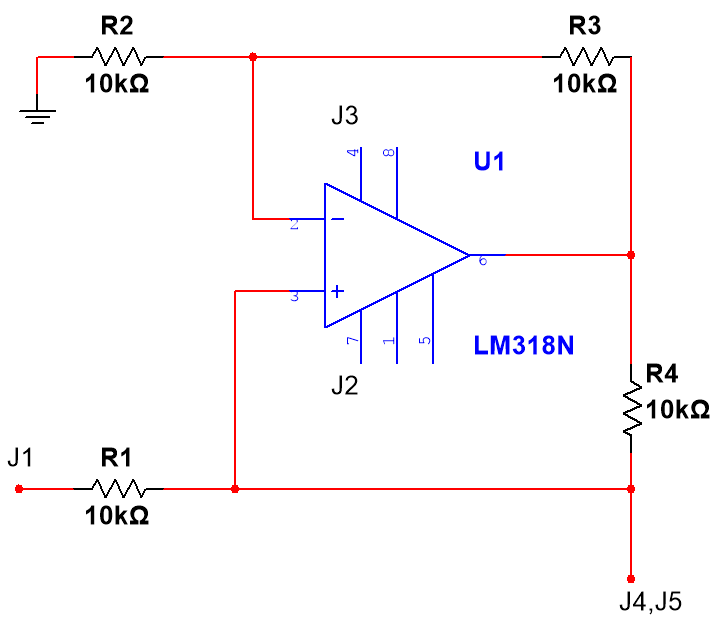
\includegraphics[width=\linewidth]
{Figure/StromgeneratorLM318.PNG}}
\caption{Figuren viser kredsløbet til strømgeneratoren LM138}
\label{Fig:GainOgfrequnecy}
\end{figure} 



\begin{equation}
\label{eq2.8}
I_{\textbf{væv}} = 2 \times \dfrac{V_{in}}{R_{5}}  $$ $$
I_{\textbf{væv(p - p)}} = 2 \times \dfrac{4_{vp}}{10k}=800uA
\end{equation}
Dette resultat omregnes til rms:
 
\begin{equation}
\label{eq2.8}
I_{\textbf{(peak)}} = \dfrac{I_{\textbf{væv(p - p)}}}{2}=400uA
$$ $$
I_{\textbf{rms}} = \dfrac{I_{\textbf{(peak)}}}{\sqrt{2}}=283uA
\end{equation}

Denne konstant strøm sendes til måleobjektets væv. 

\subsection{OP-AMP}
Outputtet af instrumentationsforstærker 2 skal yderligere forstærkes og dette sker ved at benytte en ikke-inverterende operationsforstærker som ser således ud: 

\begin{figure}[H]
\centering
{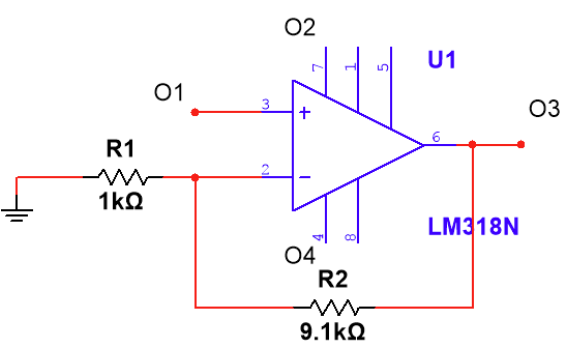
\includegraphics[width=\linewidth]
{Figure/IkkeInviterendeOpAmp}}
\caption{Figuren viser kredsløbet til strømgeneratoren LM138}
\label{Fig:GainOgfrequnecy}
\end{figure} 




Det er nødvendigt at forstærke signalet til denne størrelse, da man vil udnytte A/D konverterens inputområde, som ligger mellem $\pm 25$ \citep{NI}. Man kunne også vælge at udnytte hele A/D konverterens dynamikområde, men det er valgt at give A/D konverteren en buffer for at imødekomme signaler, der har en markant afvigelsesprocent. Hvis disse type signaler forekommer og man ikke giver A/D konverteren en buffer, så mister man al data, som overskrider de 10V.   
Der benyttes operationsforstærkeren LM318 til at forstærke signalet op, hvor Gain er bestemt af forholdet mellem to modstande, $R_1$  og $R_2$: 

\begin{equation}
\label{eq2.10}
 Gain= 1 + \dfrac{R_{2}}{R_{1}} $$ $$
\end{equation}

For at forstærke signalet op til $8V$ kræver det at man gainer $V_{outINA128}$ 54 gange og vælger $R_1=1k\Omega$. 
Hermed isoleres værdien af $R_2$:

\begin{equation}
\label{eq2.11}
 54= 1 + \dfrac{R_{2}}{1k\Omega} \Rightarrow R_{2} =53k\Omega
\end{equation}
Det forventes at operationsforstærkeren forstærker $V_{outINA128}$ til $8,1V$.\


\subsection{AA filter}

or at sikre at aliasering ikke opstår, tilføjes et analog anti-aliaseringsfilter i kredsløbet, der tillader passering af frekvenser, der er mindre end Nyquist-frekvensen og dæmper frekvenser, som er højere end Nyquist-frekvensen. I dette projekt realiseres ant-aliaserings filteret som 2. ordens lavpasfilter af typen Sallen-Key  med cutoff frekvens på 50kHz. Filteret har nedenstående overføringsfunktion: 
 \\linebreak \textbf{Indsæt et billede af filtret man nu vælger}

\begin{equation}
\label{eq2.14}
 H(s)=  \dfrac{2 \times \pi \times f_{c}}{s^{2}+ 2 \times \varsigma \times (2 \times \pi \times f_{c}) s + (2 \times \pi \times f_{c})^{2} } = 0,12mV
\end{equation} 

Filtreret knækfrekvens kan bestemmes vha. denne formel: 
\begin{equation}
\label{eq2.15}
f_{c}= \dfrac{1}{2 \times \pi \times  \sqrt{R1 \times C1 \times R2 \times C2}}
\end{equation}

I stedet for at beregne værdierne for komponenterne, anvendes et værkstøj til design af filtre, som kan regne disse komponentværdier når man indtaster den ønskede knækfrekvens 5 . Indtastning af cutoff frekvensen giver følgende resultater:

\begin{equation}
\label{eq2.16}
 R1=R2= 33k\Omega $$ $$
 C1=C2=100pF
\end{equation}

\textbf{Indsæt podeplot}
\textbf{Der mangler to punkter:
	Hvor meget er signalet dæmpede allerede?
	Hvor skal vi dæmpe det yderligere for komme ned til 100db?} 
\chapter{Software}
\subsection{Sekvens Diagram}

Sekvensdiagrammet viser rækkefølgen af programmets kodeeksekvering. Programmet igangsættes af brugeren ved ved at åbne m.filen Synkerefleksmonitor. Her ligger GUI'en til hele programmet. Brugerne kan herfra vælge at igangsætte en måling ved at trykke knappen $'Btn-Start-Measurments'$. Denne knap kører efterfølgende en række funktioner, der tilsammen måler, gemmer og viser en bioimpedans og EMG måling simultant. Hver af disse funktioner eksisterer i sin egen m.fil. Denne opdeling muliggør at man nemt kan udvide programmet uden at have kendskab til alle disse funktioner.    

\begin{figure}[H]
\centering
{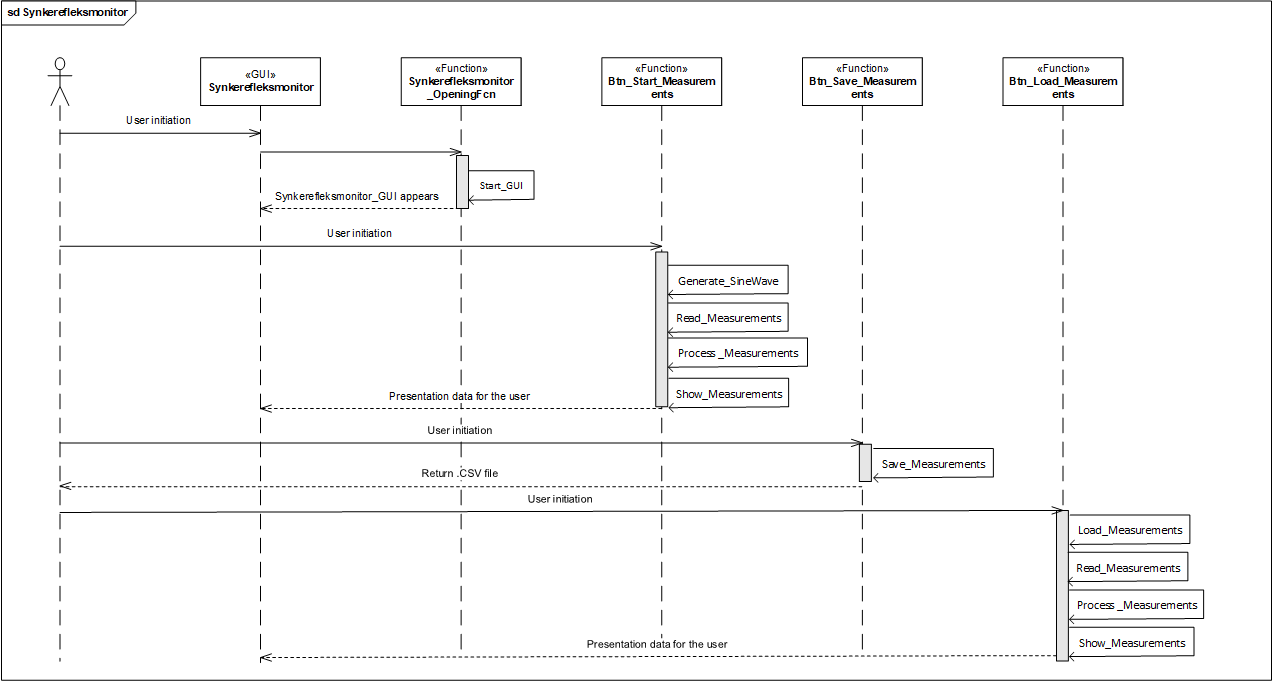
\includegraphics[width=\linewidth]
{Figure/SekevensDiagram}}
\caption{Figuren viser sekvensen af programmets kode}
\label{Fig:GainOgfrequnecy}
\end{figure} 



\bibliography{library}
\end{document}


